% \usepackage{tikz}
% \usetikzlibrary{arrows}
% \usepackage{pgfplots}
% \pgfplotsset{compat=1.3}
% \usepackage[detect-family]{siunitx}
% \usepackage[eulergreek]{sansmath}
% \sisetup{text-sf=\sansmath}

\begin{sansmath}
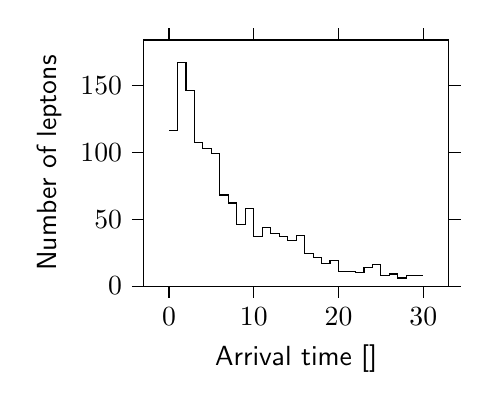
\begin{tikzpicture}[
        font=\sffamily,
        every pin/.style={inner sep=2pt, font={\sffamily\smaller}},
        every label/.style={inner sep=2pt, font={\sffamily\smaller}},
        every pin edge/.style={<-, >=stealth', shorten <=2pt},
        pin distance=2.5ex,
    ]
    \begin{axis}[
            width=.45\linewidth,
            %
            xlabel={ Arrival time [\si{\nano\second}] },
            ylabel={ Number of leptons },
            %
            xmin={  },
            xmax={  },
            ymin={ 0 },
            ymax={  },
            %
            xtick={  },
            ytick={  },
            %
            tick align=outside,
            max space between ticks=40,
            every tick/.style={},
        ]

        

        
            \addplot[no markers,solid,const plot] coordinates {
                (0.0, 116)
                (1.0, 167)
                (2.0, 146)
                (3.0, 107)
                (4.0, 103)
                (5.0, 99)
                (6.0, 68)
                (7.0, 62)
                (8.0, 46)
                (9.0, 58)
                (10.0, 37)
                (11.0, 44)
                (12.0, 39)
                (13.0, 37)
                (14.0, 34)
                (15.0, 38)
                (16.0, 24)
                (17.0, 21)
                (18.0, 17)
                (19.0, 19)
                (20.0, 11)
                (21.0, 11)
                (22.0, 10)
                (23.0, 14)
                (24.0, 16)
                (25.0, 8)
                (26.0, 9)
                (27.0, 6)
                (28.0, 8)
                (29.0, 8)
                (30.0, 8)
            };
        

        
    \end{axis}
\end{tikzpicture}
\end{sansmath}